\section{Vehicle Networking}
\subsection{Vehicle Ad-Hoc Networking (\ac{VANET})}
\ac{VANET} is a subclass of \ac{MANET}. The technology allows \ac{IVC} and is used for various reasons. With \ac{IVC}, vehicles are able to communicate with other vehicles within their vicinity. This is known as \ac{V2V}. Applications for \ac{V2V} communications include vehicle platooning and forward collision avoidance. In this survey \citep{Kiess2007OnCommunication}, it outlines a \ac{V2V} safety application. The application involves an emergency braking signal that is propagated through vehicles along the road when a vehicle suddenly stops. As vehicles behind receive this information, the vehicles themselves may be able to react on time. Other applications include speed management to avoid traffic jams and a new form of distress signal from approaching emergency vehicles.

There are other forms of \ac{VANET} models. These include \ac{V2I} and \ac{V2G}. \ac{V2I} allow vehicle communication with \ac{V2I} supported junctions, traffic lights, as well as road signs. In this paper \citep{Milanes2012AnSystem}, it proposes an \ac{ITS} through the use of \ac{V2I} communications. By proposing an intelligent traffic system, regulation of traffic flow is possible. As well as this, the system is able to monitor each vehicles' position and speed. By monitoring these characteristics, the system may alert the driver of the vehicle when it estimates a collision. Additionally, \ac{ITS} has the potential to guide autonomous vehicles through bends on the road. Road signs on road bends may act as an \ac{RSU} and notify an approaching autonomous vehicle of the speed and angle that the vehicle should approach the bend at. Alternatively, the road signs could notify the driver of the vehicle through their dashboard.

With \ac{V2G}, battery vehicles would be able to communicate with the electricity grid. Communication with the electric grid could allow vehicles to contribute to levelling the off-peak load \citep{Guille2009AImplementation}. 

\ac{VANET} models can also allow the dissemination of parking information. This can be achieved in the form of \ac{V2I}, where vehicles communicate with an \ac{RSU}. Alternatively, \ac{V2V} communications could be used to disseminate the parking data. For example, when a vehicle gives up a parking spot, it may announce as so, so that the information may be propagated to a vehicle nearby looking for a space.

An increasing amount of vehicles are being equipped with on-board wireless communication units in order to facilitate wireless network among vehicles and their environments \citep{Lin2008SecurityNetworks}. Thus more vehicles on the road could have the potential to support a smart parking system network environment.

In another paper \citep{Panayappan2007VANET-basedAvailability}, the proposal brought forward involves an urban area dissected in the form of a Voronoi diagram. This is illustrated in figure \ref{figure:voronoi}.

\begin{figure}[H]
    \centering
    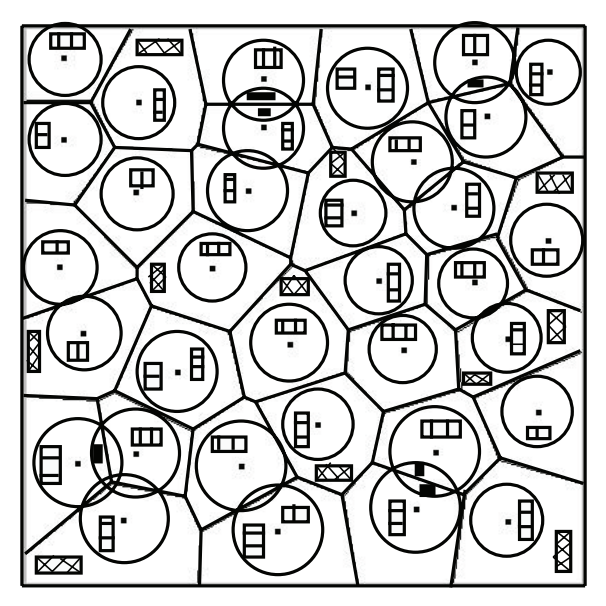
\includegraphics[width=0.35\linewidth]{./Images/VORONOI.png}
    \caption{Voronoi Model}
    \label{figure:voronoi}
\end{figure}

The paper proposes that a road side unit \ac{RSU} should be placed at the center of each individual sector in the Voronoi diagram. The \ac{RSU} is responsible for handling all the information regarding parking information within its corresponding sector. In other words, each unit is able to respond with the occupancy levels of the parking spaces in their designated sectors. Vehicles approaching a designated sector will be able to communicate with the appropriate \ac{RSU} in order to query the parking space available within that sector. The drawbacks to this implementation would be the cost. Not only must parking sensors be fitted in parking locations, on top of this, a corresponding \ac{RSU} must be placed in each sector.

\subsection{Vehicular Cloud Computing (VCC)}
Vehicular Cloud Computing \ac{VCC} can be defined as a new paradigm in which vehicles interact and collaborate to sense the environment, process the data, propagate the results and more generally share resources \citep{Mehmood2017Cyber-PhysicalCommunications}. \ac{VANET} models require \ac{OBU} to process more and more information. As highlighted in this survey \citep{Whaiduzzaman2014AComputing}, vehicles are expected to carry more storage, processing power and sensing capabilities. \ac{VCC} provides a solution to the influx of processing power required for \ac{OBU} of vehicles. Additionally, vehicular sensing capabilities can be further enhanced through the use of the cloud. Often underutilised vehicle sensors could provide real-time environment information.

In this paper \citep{Hussain2012RethinkingComputing}, it proposes three different cloud architectures. These architectures are \ac{VC}, \ac{VuC}, and \ac{HC}. In \ac{VC}, the vehicles themselves form the cloud. The pooling of resources are performed between the vehicles themselves. The most appropriate example for \ac{VC} is traffic light coordination. If there is vehicle build-up within a particular area, then vehicles in that area are able to communicate with each other and with the traffic light infrastructure to dynamically adjust junctions in real-time. In \ac{VuC}, \ac{RSU} are introduced and act as gateways to the cloud services. The cloud services provided could give vehicles access to real-time traffic information. The final cloud architecture is \ac{HC}, it is the combination of the \ac{VC} and \ac{VuC} architectures.

To conclude, with the introduction of \ac{VANET}, there is concern for the required processing power of vehicles' \ac{OBU} and underutilised capabilities of vehicle sensors and storage. The introduction of \ac{VCC} could provide a viable solution in solving these \ac{VANET} matters.